\chapter{Resultados} \label{cap:resultados}

Este capítulo apresenta os resultados obtidos e discute as implicações do estudo comparativo. Os resultados são apresentados em tabelas e gráficos, seguidos de uma análise detalhada do que fora observado. A seção é dividida em subseções que abordam os diferentes cenários de classificação, trazendo uma discussão sobre vantagens e desvantagens de cada abordagem.

\subsection{Classificação em Cinco Classes}

Para o cenário de classificação em cinco classes, os resultados das métricas de desempenho geral dos modelos de RNCs e ViTs são apresentados na \autoref{tab:overall_metrics_all_models}. A acurácia geral variou de 0.6894 a 0.7885, com o modelo DenseNet-169 alcançando a maior acurácia com uso da entropia cruzada. Considerando a característica ordinal da classificação, a métrica QWK oferece uma visão mais precisa do desempenho dos modelos. O modelo DenseNet-121 obteve o melhor QWK de 0.8878, seguido pelo GCViT-B com QWK de 0.8832, ambos com uso da entropia cruzada.

Ao avaliar o impacto da função de perda no desempenho, observou-se que, na maioria dos casos, modelos treinados usando entropia cruzada superaram seus equivalentes treinados com a CORN em termos de acurácia. Na média, houve uma queda de x\% na acurácia geral, sugerindo que a função de perda CORN pode não ser tão eficaz na previsão de classes corretas. No entanto, a CORN melhorou consistentemente o QWK para a maioria dos modelos (x\%). O modelo Inception-v3, por exemplo, teve uma melhoria de 0.8571 para 0.8813. Quanto ao MAE, também houve uma leve redução com uso da CORN, confirmando sua eficácia em reduzir a distância entre predições incorretas. Portanto, caso o objetivo seja maximizar o número de classes corretamente previstas, a entropia cruzada pode ser a melhor escolha. No entanto, para uma ferramenta de suporte à decisão clínica, onde a predição de uma classe 2 para uma classe 3 é menos grave do que prever para uma classe 0, a função de perda CORN é mais adequada, pois isso produz modelos que realizam predições mais próximas do rótulo real, mesmo que não sejam exatamente corretas.

% A \autoref{tab:resultados} mostra a acurácia dos modelos de RNCs e ViTs treinados para a classificação da OA de joelho usando a função de perda \textit{crossentropy}. Em relação ao tempo de treinamento, é possível notar que o modelo mais rápido foi o ResNet-50, com um tempo de 11.29 segundos. Por outro lado, o modelo mais lento foi o DeiT, com um tempo de 79.5 segundos. Tais valores não necessariamente indicam que o modelo mais rápido é o pior, ou o contrário, mas é importante considerar o tempo de treinamento como um fator relevante ao escolher um modelo, especialmente se houver restrições de recursos computacionais. O tempo de treinamento mostrado varia, principalmente, com o número de épocas, já que modelos que levaram mais tempo são aqueles que tiveram a parada antecipada mais tarde, ou executaram as 30 épocas completas.

\begin{table}[ht]
    \centering
    \begin{tabular}{llccc}
        \toprule
        \textbf{Modelo} & \textbf{Função de perda} & \textbf{Acurácia} & \textbf{QWK} & \textbf{MAE} \\
        \midrule
        ResNet-34 & \text{Entropia cruzada} & 0.7258 & 0.8475 & 0.3282 \\
        ResNet-34 & \text{CORN} & 0.7203 & 0.8568 & 0.3194 \\
        ResNet-50 & \text{Entropia cruzada} & 0.7478 & 0.8509 & 0.3095 \\
        ResNet-50 & \text{CORN} & 0.7379 & 0.8779 & 0.2874 \\
        ResNet-101 & \text{Entropia cruzada} & 0.7445 & 0.8556 & 0.3040 \\
        ResNet-101 & \text{CORN} & 0.7214 & 0.8633 & 0.3128 \\
        VGG-16 & \text{Entropia cruzada} & 0.7159 & 0.8534 & 0.3293 \\
        VGG-16 & \text{CORN} & 0.7115 & 0.8614 & 0.3216 \\
        VGG-19 & \text{Entropia cruzada} & 0.7048 & 0.8522 & 0.3370 \\
        VGG-19 & \text{CORN} & 0.7037 & 0.8596 & 0.3260 \\
        DenseNet-121 & \text{Entropia cruzada} & 0.7709 & \textbf{0.8878} & 0.2599 \\
        DenseNet-121 & \text{CORN} & 0.7357 & 0.8830 & 0.2852 \\
        DenseNet-169 & \text{Entropia cruzada} & \textbf{0.7885} & 0.8811 & \textbf{0.2522} \\
        DenseNet-169 & \text{CORN} & 0.7324 & 0.8767 & 0.2919 \\
        Inception-v3 & \text{Entropia cruzada} & 0.7247 & 0.8571 & 0.3172 \\
        Inception-v3 & \text{CORN} & 0.7533 & 0.8813 & 0.2742 \\
        Google-ViT-B & \text{Entropia cruzada} & 0.6938 & 0.8296 & 0.3634 \\
        Google-ViT-B & \text{CORN} & 0.6894 & 0.8442 & 0.3502 \\
        DeiT-Distilled-B & \text{Entropia cruzada} & 0.6938 & 0.8321 & 0.3634 \\
        DeiT-Distilled-B & \text{CORN} & 0.6960 & 0.8514 & 0.3381 \\
        DaViT-B & \text{Entropia cruzada} & 0.7709 & 0.8758 & 0.2687 \\
        DaViT-B & \text{CORN} & 0.7357 & 0.8700 & 0.2974 \\
        MaxViT-T & \text{Entropia cruzada} & 0.7467 & 0.8778 & 0.2841 \\
        MaxViT-T & \text{CORN} & 0.7456 & 0.8800 & 0.2819 \\
        GCViT-B & \text{Entropia cruzada} & 0.7555 & 0.8832 & 0.2742 \\
        GCViT-B & \text{CORN} & 0.7335 & 0.8804 & 0.2896 \\
        Swin-B & \text{Entropia cruzada} & 0.7059 & 0.8463 & 0.3425 \\
        Swin-B & \text{CORN} & 0.7026 & 0.8617 & 0.3293 \\
        \bottomrule
    \end{tabular}
    \caption{Métricas de desempenho de cada modelo na tarefa de classificar a OA de joelho em cinco classes, usando as funções de perda entropia cruzada e CORN.}
    \label{tab:overall_metrics_all_models}
\end{table}

A \autoref{tab:f1_scores_all_models} apresenta as métricas F1-score para cada uma das cinco classes e revela um desafio significativo na classificação da classe KL 1, que representa o estágio duvidoso da OA de joelho. O valor do F1-score entre todos os modelos e funções de perda é drasticamente menor do que para as outras classes, variando de 0.3750 (VGG-19) a 0.5970 (DenseNet-169). Esta baixa performance na classe KL 1 sugere fortemente que suas características visuais são mais difíceis de serem distinguidas das classes adjacentes, levando a uma baixa concordância entre as predições. Isso valida o estudo experimental que exclui a categoria "duvidosa".

\begin{sidewaystable}[ht]
    \centering
    \begin{tabular}{llcccccc}
        \toprule
        \textbf{Modelo} & \textbf{Função de perda} & \textbf{Macro avg} & \textbf{Grade 0} & \textbf{Grade 1} & \textbf{Grade 2} & \textbf{Grade 3} & \textbf{Grade 4} \\
        \midrule
        ResNet-34 & \text{Entropia cruzada} & 0.7384 & 0.7932 & 0.4669 & 0.7187 & 0.8465 & 0.8667 \\
        ResNet-34 & \text{CORN} & 0.7431 & 0.8034 & 0.5117 & 0.6837 & 0.8354 & 0.8814 \\
        ResNet-50 & \text{Entropia cruzada} & 0.7722 & 0.7983 & 0.5257 & 0.7364 & 0.8852 & 0.9153 \\
        ResNet-50 & \text{CORN} & 0.7564 & 0.8239 & 0.5158 & 0.7244 & 0.8326 & 0.8852 \\
        ResNet-101 & \text{Entropia cruzada} & 0.7726 & 0.7983 & 0.5683 & 0.7277 & 0.8534 & 0.9153 \\
        ResNet-101 & \text{CORN} & 0.7359 & 0.8142 & 0.4932 & 0.6920 & 0.8412 & 0.8387 \\
        VGG-16 & \text{Entropia cruzada} & 0.7276 & 0.8063 & 0.4201 & 0.6912 & 0.8537 & 0.8667 \\
        VGG-16 & \text{CORN} & 0.7384 & 0.7935 & 0.4358 & 0.7042 & 0.8583 & 0.9000 \\
        VGG-19 & \text{Entropia cruzada} & 0.7066 & 0.7898 & 0.3750 & 0.7146 & 0.8468 & 0.8070 \\
        VGG-19 & \text{CORN} & 0.7268 & 0.7935 & 0.4216 & 0.6949 & 0.8667 & 0.8571 \\
        DenseNet-121 & \text{Entropia cruzada} & 0.7777 & 0.8454 & 0.5378 & 0.7537 & 0.8807 & 0.8710 \\
        DenseNet-121 & \text{CORN} & 0.7563 & 0.8192 & 0.4890 & 0.7292 & 0.8439 & 0.9000 \\
        DenseNet-169 & \text{Entropia cruzada} & 0.8061 & 0.8384 & 0.5970 & 0.7780 & 0.9016 & 0.9153 \\
        DenseNet-169 & \text{CORN} & 0.7583 & 0.8066 & 0.5433 & 0.7097 & 0.8608 & 0.8710 \\
        Inception-v3 & \text{Entropia cruzada} & 0.7487 & 0.7959 & 0.4734 & 0.7166 & 0.8455 & 0.9123 \\
        Inception-v3 & \text{CORN} & 0.7811 & 0.8067 & 0.5464 & 0.7589 & 0.8780 & 0.9153 \\
        Google-ViT-B & \text{Entropia cruzada} & 0.7204 & 0.7599 & 0.4307 & 0.6842 & 0.8502 & 0.8772 \\
        Google-ViT-B & \text{CORN} & 0.7277 & 0.7589 & 0.4589 & 0.6781 & 0.8571 & 0.8852 \\
        DeiT-Distilled-B & \text{Entropia cruzada} & 0.7206 & 0.7670 & 0.3938 & 0.6790 & 0.8631 & 0.9000 \\
        DeiT-Distilled-B & \text{CORN} & 0.7378 & 0.7527 & 0.4230 & 0.7157 & 0.8852 & 0.9123 \\
        DaViT-B & \text{Entropia cruzada} & 0.7968 & 0.8111 & 0.5401 & 0.7807 & 0.9212 & 0.9310 \\
        DaViT-B & \text{CORN} & 0.7622 & 0.7912 & 0.4756 & 0.7510 & 0.8807 & 0.9123 \\
        MaxViT-T & \text{Entropia cruzada} & 0.7649 & 0.8329 & 0.4986 & 0.7143 & 0.8787 & 0.9000 \\
        MaxViT-T & \text{CORN} & 0.7728 & 0.8333 & 0.4945 & 0.7100 & 0.8952 & 0.9310 \\
        GCViT-B & \text{Entropia cruzada} & 0.7720 & 0.8409 & 0.5128 & 0.7136 & 0.8926 & 0.9000 \\
        GCViT-B & \text{CORN} & 0.7459 & 0.8093 & 0.4501 & 0.7463 & 0.8760 & 0.8475 \\
        Swin-B & \text{Entropia cruzada} & 0.7237 & 0.7944 & 0.4037 & 0.6795 & 0.8595 & 0.8814 \\
        Swin-B & \text{CORN} & 0.7261 & 0.7994 & 0.4261 & 0.6681 & 0.8405 & 0.8966 \\
        \bottomrule
    \end{tabular}
    \caption{Métrica F1-score para cada uma das cinco classes e modelo, usando as funções de perda entropia cruzada e CORN.}
    \label{tab:f1_scores_all_models}
\end{sidewaystable}

Modelos como o DaViT-B (CE) e GCViT-B (CE) também apresentam resultados promissores, alcançando acurácia de 0.7709 e 0.7555, respectivamente, com QWK de 0.8758 e 0.8832. Esses resultados indicam que os modelos de ViT podem ser competitivos com as RNCs tradicionais, especialmente em tarefas de classificação ordinal. No entanto, ao observar o custo computacional pela \autoref{tab:computational_performance}, nota-se que esses modelos de ViT são mais pesados em termos de FLOPs (15.28 GMac e 13.89 GMac) e parâmetros (86.93 M e 89.3 M), o que impacta no tempo de treinamento. Nesse sentido, arquiteturas da família DenseNet demonstram ser mais eficientes, com o DenseNet-169 usando apenas 12.49 M de parâmetros e 3.44 GMac FLOPs, ou seja, seis quatro menos parâmetros FLOPs do que o DaViT-B (CE).

\begin{table}[ht]
    \centering
    \begin{tabular}{lccc}
        \toprule
        \textbf{Modelo} & \textbf{Tempo (min)} & \textbf{FLOPs (GMac)} & \textbf{Parâmetros (M)} \\
        \midrule
        ResNet-34 CE & 33.46 & 3.68 & 21.29 \\
        ResNet-34 CORN & 89.29 & 3.68 & 21.29 \\
        ResNet-50 CE & 14.55 & 4.13 & 23.52 \\
        ResNet-50 CORN & 9.87 & 4.13 & 23.52 \\
        ResNet-101 CE & 22.02 & 7.86 & 42.51 \\
        ResNet-101 CORN & 16.94 & 7.86 & 42.51 \\
        VGG-16 CE & 37.70 & 19.63 & 138.36 \\
        VGG-16 CORN & 28.45 & 19.63 & 138.36 \\
        VGG-19 CE & 39.32 & 19.69 & 139.64 \\
        VGG-19 CORN & 34.68 & 19.69 & 139.64 \\
        DenseNet-121 CE & 12.74 & 2.9 & 6.96 \\
        DenseNet-121 CORN & 9.22 & 2.9 & 6.96 \\
        DenseNet-169 CE & 15.06 & 3.44 & 12.49 \\
        DenseNet-169 CORN & 16.72 & 3.44 & 12.49 \\
        Inception-v3 CE & 12.52 & 2.85 & 25.12 \\
        Inception-v3 CORN & 14.39 & 2.85 & 25.12 \\
        Google-ViT-B CE & 68.52 & 16.87 & 85.8 \\
        Google-ViT-B CORN & 35.45 & 16.87 & 85.8 \\
        DeiT-Distilled-B CE & 77.31 & 16.95 & 85.8 \\
        DeiT-Distilled-B CORN & 40.20 & 16.95 & 85.8 \\
        DaViT-B CE & 57.83 & 15.28 & 86.93 \\
        DaViT-B CORN & 27.08 & 15.28 & 86.9 \\
        MaxViT-T CE & 28.03 & 5.48 & 30.41 \\
        MaxViT-T CORN & 29.36 & 5.48 & 30.41 \\
        GCViT-B CE & 49.57 & 13.89 & 89.3 \\
        GCViT-B CORN & 34.65 & 13.89 & 89.3 \\
        Swin-B CE & 46.61 & 10.55 & 86.75 \\
        Swin-B CORN & 36.02 & 10.55 & 86.75 \\
        \bottomrule
    \end{tabular}
    \caption{Computational performance for all models and loss functions (5-class classification).}
    \label{tab:computational_performance}
\end{table}

De modo geral, os resultados indicam que os modelos de RNCs superaram os modelos de ViT, especialmente em termos de acurácia. Modelos como DenseNet-169, DenseNet-121 e Inception-v3 se destacaram, com acurácias gerais de 78.87\%, 77.09\% e 75.33\%, respectivamente. Os modelos de ViT, como DaViT-B e GCViT-B, também apresentaram resultados competitivos, com acurácias de 77.09\% e 75.55\%. No entanto, a performance de QWK foi muito próxima entre os modelos, indicando que ambas as arquiteturas são capazes de entender a natureza ordinal da classificação da OA de joelho e evitar erros significativos.

% Quanto à acurácia geral (\textit{overall}), todos os modelos apresentaram resultados razoavelmente bons, com valores variando de 0.6723 a 0.7319. Isso indica que todos os modelos foram capazes de aprender padrões relevantes para a classificação da OA de joelho. No entanto, é importante notar que o modelo DenseNet-169 obteve a maior acurácia geral, com um valor de 0.7319. Isso sugere que arquiteturas de RNCs densamente conectadas podem ser muito eficazes na extração de características relevantes em imagens médicas como radiografias de joelho. Além disso, os modelos de conexões residuais (ResNet) também apresentaram resultados competitivos, com acurácias gerais variando de 0.7044 a 0.7248, onde o ResNet-50 obteve a maior acurácia dentre eles e com o menor tempo de treinamento, oferecendo um bom equilíbrio entre generalização do modelo e custo computacional.

% Por outro lado, os modelos da família VGG (VGG-16 e VGG-19) apresentaram acurácias gerais mais baixas, variando de 0.6723 a 0.6851, o que sugere que essas arquiteturas mais simples podem não ser tão eficazes na extração de características complexas em radiografias de joelho. Embora fosse esperado que esses modelos tivessem desempenho inferior em relação aos modelos ResNet, devido à sua profundidade, os resultados indicam que esses modelos são capazes de aprender padrões relevantes e ter uma menor probabilidade de \textit{overfitting}, como observado no tempo de treinamento do VGG-16, que foi maior que a maioria dos modelos justamente por não ter parada antecipada em virtude da queda do erro no conjunto de validação.

% O GoogLeNet, com sua arquitetura Inception (versão 3), permitiu que o modelo tivesse uma acurácia geral de 0.7215, indicando que o modelo pode ser eficaz na extração de características relevantes e superar a maioria dos modelos de RNCs. Esse comportamento pode ser justificado pelo uso de uma técnica chamada de "bottleneck" ou "redução de dimensionalidade", que reduz a quantidade de parâmetros e a complexidade computacional do modelo, sem comprometer significativamente o desempenho.

% Os modelos de transformers, por sua vez, apresentaram acurácias gerais variando de 0.6862 a 0.7215, indicando que essas arquiteturas podem ser eficazes, mas talvez não sejam tão eficientes quanto os modelos de RNCs. O modelo Swin Transformer obteve a maior acurácia geral entre os modelos de transformers, com um valor de 0.6977, sugerindo que a abordagem hierárquica de atenção pode ser eficaz na extração de características relevantes em radiografias de joelho.

% Entretanto, é importante notar que a acurácia para a classe KL 1 foi baixa para todos os modelos, variando de 0.2562 e 0.4475. Isso indica que a classificação da OA de joelho no estágio 1 (duvidoso) pode ser mais desafiadora, possivelmente devido à semelhança visual com as classes adjacentes KL 0 e KL 2. Esse resultado pode ser observado na \autoref{confusion-matrix-resnet50}, que mostra a matriz de confusão do modelo ResNet-50. A classe KL 1 tem a menor acurácia dentre todas as classes, o que reflete o desafio na classificação dessa classe devido ao nível de detalhe ou até mesmo incoerência no rotulação das imagens do dataset.

% \begin{figure}
%     \centering
%     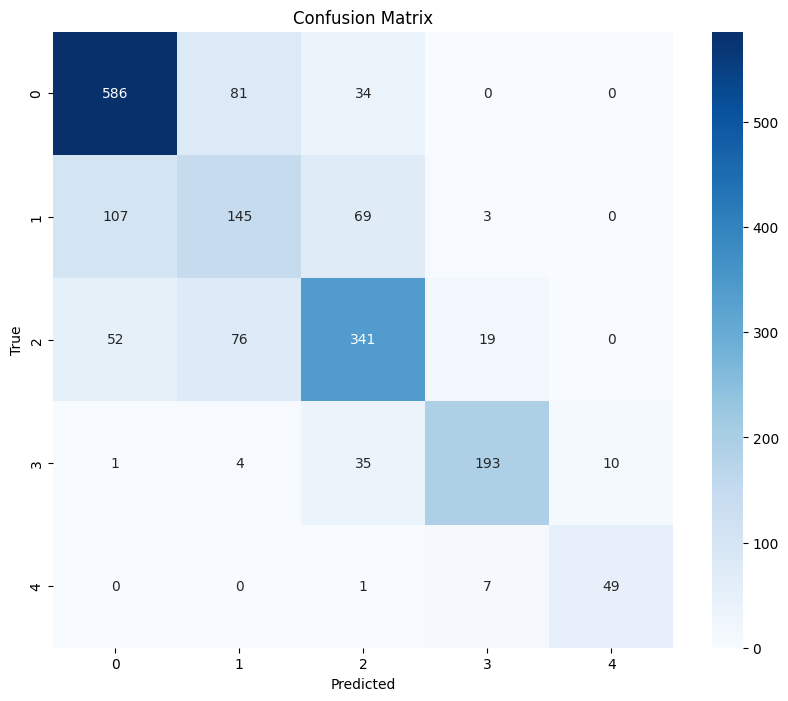
\includegraphics[width=\linewidth]{figs/confusion-matrix-resnet50.png}
%     \caption{Matriz de confusão do modelo ResNet-50.}
%     \label{confusion-matrix-resnet50}
% \end{figure}

% Em resumo, os modelos ResNet-50 e DenseNet-169 se destacaram em termos de tempo de treinamento e acurácia geral, respectivamente. No entanto, é importante considerar as características de cada classe ao escolher um modelo, pois diferentes modelos podem ter desempenhos diferentes para cada classe.

% A \autoref{tab:resultados-corn} apresenta os resultados dos modelos de RNCs e ViTs treinados para a classificação da OA de joelho usando a função de perda CORN. Em relação ao tempo de treinamento, não houve uma mudança significativa comparado com a função de perda \textit{crossentropy}. O modelo mais rápido foi, novamente, o ResNet-50, com um tempo de 10.32 segundos, enquanto o modelo mais lento foi o Swin Transformer, com um tempo de 35.58 segundos. Em relação à acurácia geral, os resultados variaram de 0.6546 a 0.7181, indicando que a função de perda CORN pode ser eficaz na classificação da OA de joelho, mas não necessariamente supera a função de perda \textit{crossentropy}. Isso é justificado pelo fato de que a função de perda CORN é mais adequada quando o modelo faz predições mais afastadas do rótulo real, o que não foi evidenciado ao observar as matrizes de confusão dos modelos.

% \begin{table}
%     \centering
%     \begin{tabular}{|c|c|c|c|c|c|c|c|}
%         \hline
%         \multirow{2}{*}{Modelo} & \multirow{2}{*}{Tempo} & \multirow{2}{*}{Overall} & \multicolumn{5}{|c|}{Classe KL} \\ \cline{4-8}
%         &  &  & 0 & 1 & 2 & 3 & 4 \\ \hline
%         ResNet-34 & 14.93 & 0.6895 & 0.7518 & 0.5586 & 0.6107 & 0.8107 & 0.8246 \\ \hline
%         ResNet-50 & 10.32 & 0.7181 & 0.796 & 0.5031 & 0.6824 & 0.823 & 0.8421 \\ \hline
%         ResNet-101 & 16.17 & 0.6994 & 0.7418 & 0.4506 & 0.707 & 0.8519 & 0.8772 \\ \hline
%         VGG-16 & 19.29 & 0.6762 & 0.7646 & 0.358 & 0.6824 & 0.7984 & 0.8246 \\ \hline
%         VGG-19 & 24.05 & 0.6669 & 0.7974 & 0.3549 & 0.6066 & 0.7901 & 0.8246 \\ \hline
%         DenseNet-121 & 10.62 & 0.6911 & 0.729 & 0.4444 & 0.7172 & 0.8272 & 0.8246 \\ \hline
%         DenseNet-169 & 13.75 & 0.717 & 0.7874 & 0.5833 & 0.6393 & 0.8148 & 0.8596 \\ \hline
%         Inception-v3 & 17.09 & 0.701 & 0.7932 & 0.5093 & 0.6639 & 0.7325 & 0.8421 \\ \hline
%         ViT-B & 36.97 & 0.6817 & 0.7447 & 0.4815 & 0.6393 & 0.8066 & 0.8772 \\ \hline
%         DeiT & 34.73 & 0.6602 & 0.7047 & 0.4877 & 0.6209 & 0.7984 & 0.8421 \\ \hline
%         Swin & 35.58 & 0.6546 & 0.7803 & 0.4658 & 0.6722 & 0.8395 & 0.7894 \\ \hline
%     \end{tabular}
%     \caption{Desempenho dos modelos de RNCs e ViTs na classificação da OA de joelho usando a função da perda CORN.}
%     \label{tab:resultados-corn}
%     \end{table}

% No entanto, é importante notar que o modelo ResNet-50 obteve a maior acurácia geral, com um valor de 0.7181, superando os demais modelos, inclusive o modelo DenseNet-169, que obteve a maior acurácia geral com a função de perda \textit{crossentropy}. Isso sugere que a função de perda CORN pode ser eficaz em arquiteturas de RNCs, especialmente aquelas com conexões residuais. Entretanto, o modelo DenseNet-169 foi quem obteve a maior acurácia para a classe KL 1, com um valor de 0.5833, que é a classe mais desafiadora de ser classificada, como observado anteriormente.

% \section{Resultados e Discussão}

% \subsection{Visão Geral dos Resultados}

% Os experimentos envolveram avaliação de 18 arquiteturas (CNN e ViT), cada uma treinada com duas funções de perda: \emph{cross entropy} e \emph{Corn} (cumulative ordinal regression). As métricas principais consideradas foram acurácia, kappa de Cohen (coeficiente de concordância), weighted Quadratic Weighted Kappa (QWK) e Mean Absolute Error (MAE). A Tabela~\ref{tab:resultados} resume os cinco modelos com melhor desempenho em termos de QWK, para ambas as funções de perda.

% \subsection{Discussão}

% Observa-se que o modelo \textbf{GCViT} apresentou o melhor desempenho global, atingindo QWK de 0.8725 com \emph{cross entropy} e 0.8752 com \emph{Corn}, além de MAE mínimo de 0.29399 e 0.29123, respectivamente;:contentReference[oaicite:1]{index=1}. Logo em seguida, os modelos \textbf{DaViT} e \textbf{MaxViT\_T} também se destacaram, com QWK acima de 0.86 e MAE abaixo de 0.32, evidenciando a eficácia de transformers especializados para tarefas de classificação ordinal de osteoartrite.

% Entre as CNNs, as versões densas (\emph{DenseNet169} e \emph{DenseNet121}) obtiveram desempenhos notáveis, com QWK acima de 0.85 e acurácias próximas a 72\% sob \emph{cross entropy}, mas ficaram abaixo dos ViTs em QWK e MAE;:contentReference[oaicite:3]{index=3}.

% Ainda, a função de perda \emph{Corn} mostrou ligeira melhora em QWK para a maioria dos modelos de ViT, embora com tempo de treinamento tipicamente maior do que com \emph{cross entropy} (por exemplo, GCViT: 3454\,s vs.\ 2423\,s);:contentReference[oaicite:5]{index=5}.

% \begin{table}[htb]
% \centering
% \caption{Desempenho dos cinco melhores modelos (ordem por QWK) para as duas funções de perda.}
% \label{tab:resultados}
% \begin{tabular}{l|ccccc|ccccc}
% \hline
% \multirow{2}{*}{\textbf{Modelo}} & \multicolumn{5}{c|}{\textbf{Cross Entropy}} & \multicolumn{5}{c}{\textbf{Corn}} \\
%  & Acc. & Kappa & QWK & MAE & Tempo (s) & Acc. & Kappa & QWK & MAE & Tempo (s) \\
% \hline
% GCViT        & 0.7363 & 0.6372 & 0.8725 & 0.29399 & 3454.0 & 0.7347 & 0.6369 & 0.8752 & 0.29123 & 2422.6 \\
% DaViT        & 0.7358 & 0.6362 & 0.8647 & 0.30226 & 3045.0 & 0.7286 & 0.6288 & 0.8713 & 0.29950 & 2342.1 \\
% MaxViT\_T    & 0.7220 & 0.6165 & 0.8616 & 0.31550 & 1489.6 & 0.7038 & 0.5934 & 0.8636 & 0.32267 & 1006.4 \\
% DenseNet169  & 0.7220 & 0.6158 & 0.8519 & 0.32488 &  888.2 & 0.7187 & 0.6143 & 0.8660 & 0.31219 & 1345.6 \\
% DenseNet121  & 0.7204 & 0.6110 & 0.8514 & 0.32708 & 1148.4 & 0.7071 & 0.6001 & 0.8592 & 0.32377 &  624.8 \\
% \hline
% \end{tabular}
% \end{table}

% \subsection{Principais Conclusões}

% \begin{itemize}
%   \item \textbf{GCViT} foi o modelo de melhor desempenho, com QWK máximo de 0.8752 e MAE mínimo de 0.2912, indicando superior capacidade de modelar a natureza ordinal da escala KL.
%   \item Transformers (GCViT, DaViT, MaxViT\_T) superaram consistentemente as CNNs clássicas em QWK e MAE, embora demandem maior custo computacional.
%   \item A função de perda \emph{Corn} proporcionou ganhos moderados em QWK para ViTs, justificando seu uso em tarefas de classificação ordinal.
%   \item Dentre as CNNs, \emph{DenseNet169} e \emph{DenseNet121} foram as mais competitivas, alcançando QWK acima de 0.85.
% \end{itemize}
